\documentclass{astroedu-lab}

\begin{document}

\pagestyle{plain}

\begin{problem}{\large Лабораторная работа 1.1.1}

\begin{bfseries}
	Условие:
\end{bfseries}

Определение систематических и случайных погрешностей при измерении удельного сопротивления нихромовой проволки.

\begin{bfseries}
	Цель работы:
\end{bfseries}

Измерить удельное сопротивление проволки и вычислить систематические и случайные погрешности.

\begin{bfseries}
	В работе используются:
\end{bfseries}

Линейка, штангенциркуль, микрометр, отрезок проволки из нихрома, амперметр, вольтметр, источник ЭДС, мост постоянного тока, реостат, ключ.

\begin{bfseries}
	Решение:
\end{bfseries}

2)Точность измерения при помощи штангенциркуля - 0.1мм. При помощи микрометра - 0.01 мм.

Результаты измерения диаметра проволки на 10 различных участках:

\begin{tabular}[t]{|l|l|l|l|l|l|l|l|l|l|l|}
\cline{1-11}
		   & 1 & 2 & 3 & 4 & 5 & 6 & 7 & 8 & 9 & 10\\ \cline{1-11}
$d_1$ (мм) & 0.4 & 0.4 & 0.4 & 0.4 & 0.4 & 0.4 & 0.4 & 0.4 & 0.4 & 					 0.4\\ \cline{1-11}
$d_2$ (мм) & 0.36 & 0.36 & 0.36 & 0.36 & 0.36 & 0.36 & 0.35 & 0.36 & 				 0.36 & 0.37\\ \cline{1-11}
\end{tabular}

\begin{equation}
	\overline{d_1} = 0.4
\end{equation}
\begin{equation}
	\overline{d_2} = 0.36
\end{equation}


При измерении диаметра штангенциркулем случайная погрешность отсутствует, а значит точность определяется систематической погрешностью прибора

\begin{equation}
	\overline{d_1} = (0.4 \pm 0.1) мм
\end{equation}

Случайная погрешность измерений при помощи микрометра:

\begin{equation}
	\sigma_{\text{сл}} = \frac{1}{N} \sqrt{\sum_{i=1}^{n}(d - \overline{d})^2} = 1.4 \cdot 10^{-3} \text{мм}
\end{equation}

Систематическая же:

\begin{equation}
	\sigma_{\text{сист}} = 0.01 \text{мм}
\end{equation}

Поскольку $\sigma_{\text{сл}} \ll \sigma_{\text{сист}}$, то можно считать проволку однородной по диаметру, а погрешность диаметра $\sigma_d$ равной систематической погрешности микрометра $\sigma_{\text{сист}}$.

\begin{equation}
	\sigma_d \approx \sigma_{\text{сист}} = 0.01 \text{мм}
\end{equation}

\begin{equation}
	d_2 = \overline{d_2} \pm \sigma_d = (3.6 \pm 0.1) \cdot 10^{-4} \text{м}
\end{equation}

Площадь поперечного сечения из наиболее точного замера микрометром

\begin{equation}
	S = \frac{\pi d_2^2}{4} \approx 1.02 \cdot 10^{-7} \text{м$^2$}
\end{equation}

Погрешность площади

\begin{equation}
	\sigma_S = 2 \frac{\sigma_d}{d_2}S \approx 6 \cdot 10^{-9} \text{м$^2$}
\end{equation}

Наконец $S = (1.02 \pm 0.06) \cdot 10^{-7} \text{м$^2$}$

3)Основные характеристики приборов

\begin{tabular}[t]{|l|l|l|l}
\cline{1-3}
		& Вольтметр & Амперметр \\ \cline{1-3}
Система & Цифровой & Магнитоэлектрическая \\
Класс точности & 0.001 & 0.2 \\
Предел измерений($x_{\text{п}}$) & 10 В & 0.15 А \\
Число делений шкалы(n) & $10^5$ & 150 \\
Цена деления ($x_{\text{п}}/n$) & $10^{-4}$ В & 1 мА \\
Чувствительность ($n/x_{\text{п}}$)&$10^4$ В$^{-1}$&$10^3$ А$^{-1}$ \\
Абсолютная погрешность ($\Delta x_M$)&$10^{-4}$ В&1 мА \\ 
Внутреннее сопротивление & 10 МОм & 0.5 Ом \\
\cline{1-3}
\end{tabular}

4)
Первая поправка

\begin{equation}
	\epsilon_1 = \frac{R_{\text{пр}}}{R_V} = \frac{5 \text{ Ом}}{10^7 \text{Ом}} = 5 \cdot 10^{-7}
\end{equation}

Вторая поправка

\begin{equation}
	\epsilon_2 = \frac{R_A}{R_{\text{пр}}} = \frac{0.5 \text{ Ом}}{5 \text{ Ом}} = 0.1
\end{equation}

$\epsilon_1 \ll \epsilon_2$, а значит первая схема предпочтительнее, при этом множитель с этим членом пренебрежимо близко к 1, а значит его можно не учитывать в дальнейшем

\newpage

5)Соберу схему как на рисунке

\begin{center}

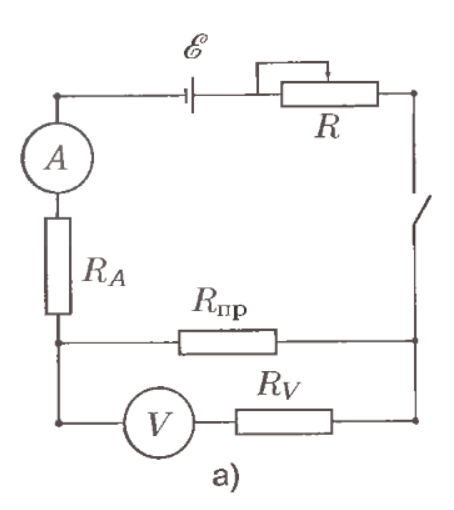
\includegraphics[width=0.3\linewidth]{pic_1.png}

\label{fig:mpr}

\end{center}
\

Показания вольтметра и амперметра

\begin{center}
\begin{tabular}[t]{|l|l||l|l||l|l|}
\hline
\multicolumn{2}{|c||}{l = 20 см} & \multicolumn{2}{|c||}{l = 30 см} & \multicolumn{2}{|c|}{l = 50 см} \\
\hline
V, В & I, мА & V, В & I, мА & V, В & I, мА \\
\hline
0.3262 & 152 & 0.4780 & 150 & 0.7730 & 146 \\
0.2700 & 125 & 0.3880 & 121 & 0.6285 & 119 \\
0.1720 & 80  & 0.3196 & 100 & 0.4740 & 90  \\
0.1290 & 60  & 0.2550 & 80  & 0.3690 & 70  \\
0.1070 & 50  & 0.1900 & 60  & 0.2643 & 50  \\
0.0650 & 30  & 0.1260 & 40  & 0.1575 & 30  \\
\hline
0.0555 & 26  & 0.0795 & 25  & 0.1826 & 35  \\
0.0860 & 40  & 0.1100 & 35  & 0.3140 & 60  \\
0.1510 & 70  & 0.1585 & 50  & 0.4230 & 80  \\
0.1948 & 90  & 0.2235 & 70  & 0.5275 & 100 \\
0.2370 & 110 & 0.2900 & 91  & 0.6330 & 120 \\
0.2795 & 130 & 0.4160 & 130 & 0.7115 & 135 \\
\hline
\end{tabular}
\end{center}

Соответствующий график

\definecolor{chucknorris}{rgb}{192,0,0}

\begin{center}
\begin{tikzpicture}
\begin{axis}[
	xlabel     = \text{I, мА}, % label x axis
    ylabel     = \text{V, В}, % label y axis
	xmin = 0, ymin = 0
	]
\addplot[mark = *] table {
	x     y
152.0 0.3262
125.0 0.27
80.0 0.172
60.0 0.129
50.0 0.107
30.0 0.065
0.0 0.0
};
\addplot[mark = +] table {
	x     y
0.0 0.0
26.0 0.0555
40.0 0.086
70.0 0.151
90.0 0.1948
110.0 0.237
130.0 0.2795
};
\addplot[mark = *] table {
	x     y
0.0 0.0
150.0 0.478
121.0 0.388
100.0 0.3196
80.0 0.255
60.0 0.19
40.0 0.126
};
\addplot[mark = +] table {
	x     y
0.0 0.0
25.0 0.0795
35.0 0.11
50.0 0.1585
70.0 0.2235
91.0 0.29
130.0 0.416
};
\addplot[mark = *] table {
	x     y
0.0 0.0
146.0 0.773
119.0 0.6285
90.0 0.474
70.0 0.369
50.0 0.2643
30.0 0.1575
};
\addplot[mark = +] table {
	x     y
0.0 0.0
35.0 0.1826
60.0 0.314
80.0 0.423
100.0 0.5275
120.0 0.633
135.0 0.7115
};
\end{axis}
\end{tikzpicture}
\end{center}

Теперь определю значение сопротивления проволки для каждой длины проволки из закона Ома $\left( R = \frac{U}{I} \right)$ и занесу результаты в таблицу

\begin{center}
\begin{tabular}[t]{|l||l||l|}
\hline
l = 20 см & l = 30 см & l = 50 см \\
\hline
$R_0 = 2.1396 \text{ Ом}$ & $R_0 = 3.1654\text{ Ом}$ & $R_0 = 5.3071\text{ Ом}$\\
$R_{\text{пр}} = 2.152\text{ Ом}$ & $ R_{\text{пр}} = 3.209\text{ Ом}$ & $ R_{\text{пр}} = 5.296\text{ Ом}$ \\
$\sigma_{R_{\text{пр}}} = 0.007\text{ Ом} $ & $ \sigma_{R_{\text{пр}}} = 0.011\text{ Ом} $ & $\sigma_{R_{\text{пр}}} = 0.018\text{ Ом}$ \\
\hline


\end{tabular}
\end{center}

Ошибка значения сопротивления составляет

\begin{equation}
	\sigma_{R_{\text{пр}}} = R_\text{пр} \sqrt{\left( \frac{\Delta x_V}{2V} \right)^2 + \left( \frac{\Delta x_I}{2I} \right)^2} = R_\text{пр} \sqrt{\left( \frac{10^{-4}\text{В}}{2 \cdot 10 \text{ В}} \right)^2 + \left( \frac{1 \text{ мА}}{2 \cdot 150 \text{ мА}} \right)^2} \approx \frac{1}{300}  R_\text{пр}
\end{equation}

Занесем полученные значения в таблицу

6)Результаты замеров мостом P4833 аналогично занесу в таблицу

Как видно, отличие замеров сопротивлений мостиком и схемой в первых 2-х замерах выходит за пределы погрешности. Это может быть обусловлено как неучтенной систематической погрешностью моста, так и плохим контактом с проволкой в разных замерах. Сильного отличия результатов нет, поэтому измерения можно считать корректными.

8)Рассчитаю удельное сопротивление по формуле

\begin{equation}
	\rho = \frac{R_\text{пр} S}{l}
\end{equation}

\begin{center}
\begin{tabular}[t]{|l|l|l|}
\hline
l, м & $\rho$, Ом$\cdot$м & $\sigma_{\rho}$, Ом$\cdot$м \\
\hline
0.2 & $1.10 \cdot 10^{-6}$ & $7 \cdot 10^{-8}$ \\
0.3 & $1.09 \cdot 10^{-6}$ & $6 \cdot 10^{-8}$ \\
0.5 & $1.08 \cdot 10^{-6}$ & $6 \cdot 10^{-8}$ \\
\hline
\end{tabular}
\end{center}

Итого $\rho = \left( 1.09 \pm 0.06 \right) \cdot 10^{-6}$ Ом$\cdot$м 

Основной вклад в погрешность результата вносит погрешность площади сечения проволки($\approx6\%$), определяющаяся погрешностью её диаметра. Поэтому для замеров сопротивления достаточно вдвое меньшей погрешности($\approx3\%$)

9)Полученное удельное сопротивление соответствует диапазону удельных сопротивлений нихрома $\left(1.05-1.4\right) \text{Ом$\cdot$мм$^2$/м}$, с большой вероятностью это один из самых распространенных, сплав Х20Н80.

Удельное сопротивление найдено, а значит цель работы достигнута.
	

\end{problem}
\end{document}